
\section{Resultados}

\subsection{Red de interacciones y robustez}

La siguiente imagen (Imagen1) muestra la red de interaciones del ser humano con las proteínas del SARS-CoV. Como podemos ver el SARS-CoV interacciona con 89 proteínas humanas, produciendo un total de 475 interacciones. 
\begin{figure}
	\centering
	
		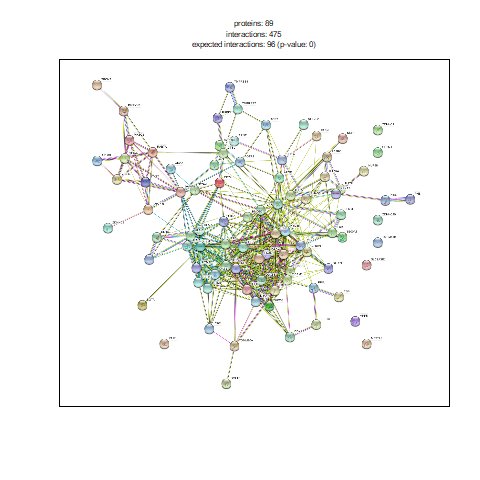
\includegraphics[width=70mm,scale=1.2]{figures/string_hits.png}
		
		\caption{\textit{Imagen1. Red de interacciones del SARS-CoV con las proteínas humanas}}
		
\end{figure}

Tras eliminar los nodos que no están conectados, hemos obtenido la red real de interacciones que podemos ver a continuación(imagen2). Sin embargo hay demasiadas conexiones como para poder distinguir los nodos. Es por ello que realizaremos los pasos siguientes de clustering, para así poder extraer la información relevante de la red. 
\begin{figure}
	\centering
	
		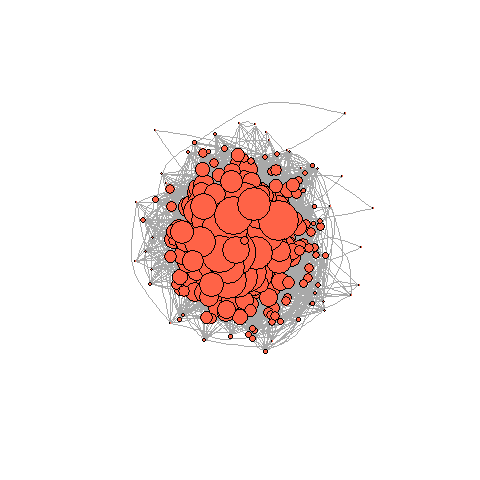
\includegraphics[width=70mm,scale=1.2]{figures/hits.network_graph.png}
		
		\caption{\textit{Imagen2. Red de interacciones del SARS-CoV con las proteínas humanas tras un proceso de filtrado}}

\end{figure}


Antes de empezar con ese proceso vamos a estudiar diferentes aspectos de nuestra red. En primer lugar si observamos la imagen(imagen3), vemos que el la distribución de grado sigue la ley de potencias, por lo tanto nuestra red sigue un modelo de free-scale, lo cual era predecible al estar tratando con una red real. 

Podemos  ver una gran cantidad de hubs. 
\begin{figure}
	\centering
	
		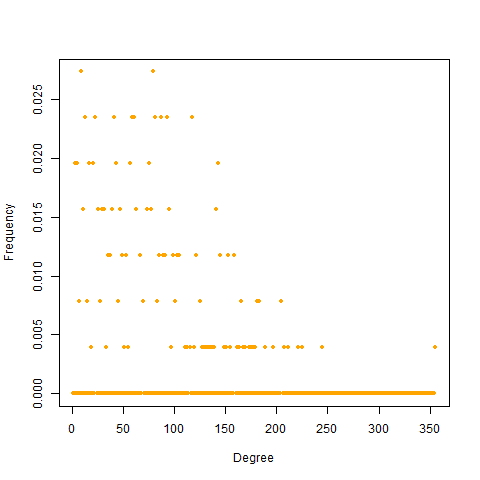
\includegraphics[width=70mm,scale=1.2]{figures/degree_distribution.png}
		
		\caption{\textit{Imagen3. Distribución de grado}}
		
\end{figure}

El coeficiente medio de agrupamiento es de 0.605, lo cual es bastante alto. Además se puede observar la característica propia de las redes reales la cual afirma que conforme el grado de los nodos aumenta, el coeficiente de agrupamiento disminuye. 

\begin{figure}
	\centering
	
	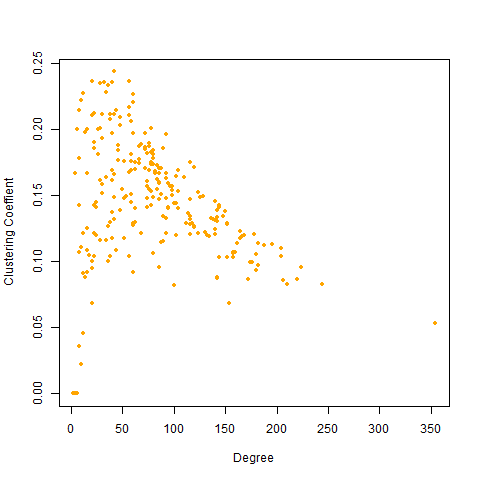
\includegraphics[width=70mm,scale=1.2]{figures/coeficiente_agrupamiento.png}
	
	\caption{\textit{Imagen4. Coeficiente de Agrupamiento}}
	
\end{figure}


Al observar la distancia entre nodos, 
\begin{figure}
	\centering
	
	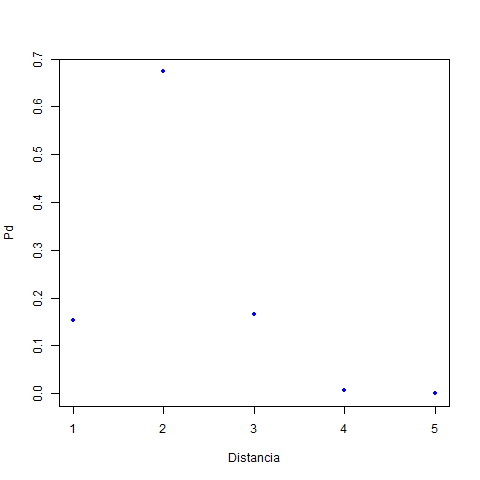
\includegraphics[width=70mm,scale=1.2]{figures/distancia.png}
	
	\caption{\textit{Imagen4. Coeficiente de Agrupamiento}}
	
\end{figure}

Para poder estudiar cual es la capacidad de nuestra red de mantener sus funciones frente a la presencia de "ataques" y ver cuán de adaptable es, usamos la robustez. Podemos observar que para ataques aleatorios es bastante robusta, mientras que para ataques dirigidos es más débil. 

\begin{figure}
	\centering
		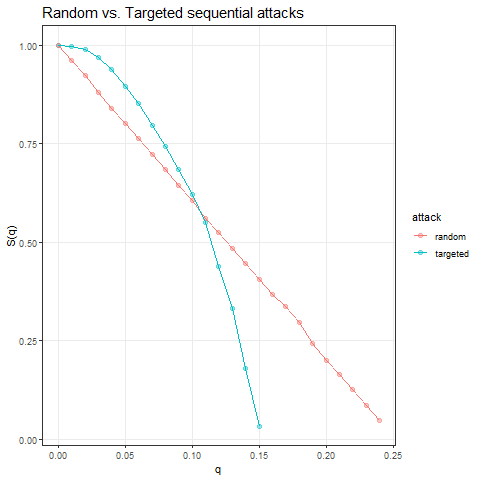
\includegraphics[width=70mm,scale=1.2]{figures/sequential_attacks.png}
		\caption{\textit{Robustez frente a ataques dirigidos y aleatorios}}
\end{figure}

\subsection{Clustering}




